\documentclass[11pt,a4paper]{article}
\usepackage[utf8]{inputenc}
\usepackage[T1]{fontenc}
\usepackage{geometry}
\geometry{a4paper, margin=1in}
\usepackage{amsmath, amssymb, amsthm}
\usepackage{graphicx}
\usepackage{hyperref}
\usepackage{booktabs}
\usepackage{cite}
\usepackage{algorithm}
\usepackage{algpseudocode}

\title{HIN1: A Hybrid Inference Network for Abstract Reasoning via Parallel Pseudo-Reinforcement Learning and Multi-Tensor VAE Test-Time Optimization}
\author{Seungwon Lee \\ \texttt{seungwon@example.com}}
\date{\today}

\begin{document}

\maketitle

\begin{abstract}
The Abstraction and Reasoning Corpus (ARC) challenges artificial general intelligence by requiring fluid reasoning and adaptation to novel tasks with extremely sparse examples. We introduce \textbf{HIN1 (Hybrid Inference Network 1)}, a two-phase architecture designed to bridge the gap between global pattern synthesis and local task-specific adaptation. Phase 1 employs a \textbf{Pseudo-Reinforcement Learning (Pseudo-RL)} framework, where a transformer-based agent iteratively refines its reasoning trajectories through self-supervised rollout generation and a \textbf{Unified Training Scheduler}. Phase 2 introduces an \textbf{Evolutionary Test-Time Compute (TTC)} phase, utilizing a specialized \textbf{MultiTensorSystem (MTS)} and a Variational Autoencoder (\textbf{VAE}) to perform per-task latent space optimization. Our approach leverages high-throughput GPU parallelization to orchestrate multiple training iterations, achieving significant performance gains on the ARC-AGI benchmark by grounding abstract logic in a structured, multi-dimensional tensor environment.
\end{abstract}

\section{Introduction}
The Abstraction and Reasoning Corpus (ARC) \cite{chollet2019measure} serves as a benchmark for "fluid intelligence," necessitating the ability to generalize from a few examples to an unseen test grid. Traditional deep learning models, despite their scale, often fail to capture the underlying symbolic and spatial logic of ARC due to their reliance on static inference pathways.

To address these challenges, we present \textbf{HIN1}, a Hybrid Inference Network that operationalizes test-time adaptation (TTA) and iterative self-improvement. HIN1 combines the strengths of large-scale offline pre-computation with rigorous, task-specific online refinement, ensuring that the model not only recognizes patterns but actively optimizes its internal representations to fit the unique constraints of each ARC puzzle.

\section{The HIN1 Architecture}
HIN1 is characterized by its two-stage operational lifecycle: an offline trajectory-based synthesis phase and an online gradient-based refinement phase (see Figure \ref{fig:arch}).

\begin{figure}[htbp]
    \centering
    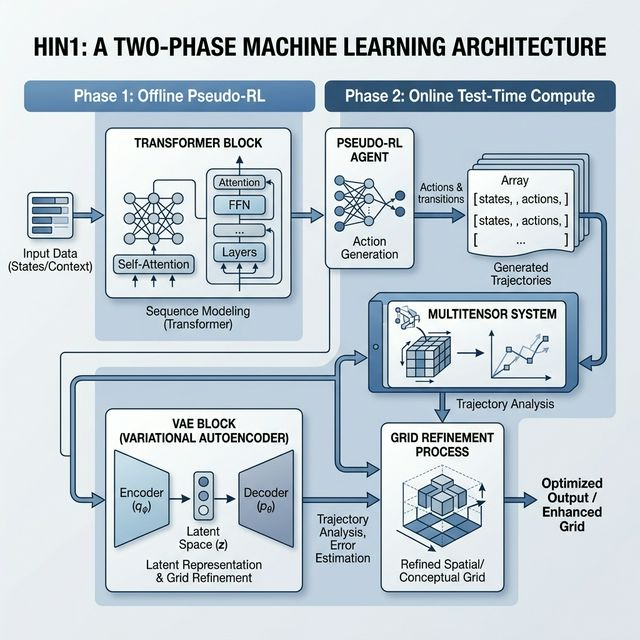
\includegraphics[width=0.9\linewidth]{conceptual_architecture.png}
    \caption{Conceptual architecture of HIN1 showing the dual-phase optimization loop.}
    \label{fig:arch}
\end{figure}

\subsection{Phase 1: Offline Pseudo-RL Synthesis}
The first phase focuses on building a generalizable "reasoning synthesizer." We utilize a \textbf{Pseudo-Reinforcement Learning} loop that treats the model's own exploratory attempts as a source of high-quality training data. 

\textbf{Unified Training Scheduler}: To manage the complexity of multi-iteration training, we implement a custom scheduler that synchronizes learning rate decays and warmup cycles across 24-hour production runs. This ensures stable convergence as the model transitions from initial supervised learning to mixed-modality training with self-generated trajectories.

\textbf{Model Backbone}: The synthesizer is a Transformer-based architecture (8 layers, 8 heads, 768 embedding dimensions) optimized with \textbf{FlashMultiheadAttention} and \textbf{MultiQueryAttention (MQA)}. MQA significantly reduces the memory footprint during the rollout generation phase, enabling high-throughput trajectory sampling.

\subsection{Phase 2: Online Evolutionary Test-Time Compute}
Phase 2 adapts the HIN1 synthesizer to the specific requirements of a given ARC task. This is achieved through an iterative optimization process localized within the task's specific grid dimensions.

\textbf{MultiTensorSystem (MTS)}: At the heart of the test-time adaptation is the MTS, a 5D tensor architecture that manages state across dimensions of examples, colors, spatial directions, and resolution. MTS provides the necessary abstractions for performing complex grid transformations (e.g., directional sharing, shifts, and symmetry-aware operations) as first-class tensor operations.

\textbf{VAE-Based Refinement}: We utilize an \textbf{ARCCompressor} (Variational Autoencoder) to model the latent space of the task. During test-time, the model weights and latent distributions are optimized using the \textbf{Adam optimizer} for up to 2000 iterations. This process, termed "Evolutionary Test-Time Compute," involves maintaining an Exponential Moving Average (EMA) of candidate solutions and selecting the most frequent, high-scoring reconstructions as final predictions.

\section{Conclusion}
HIN1 represents a scalable framework for approaching abstract reasoning through the lens of hybrid optimization. By partitioning the problem into global reasoning synthesis (Pseudo-RL) and local task refinement (MTS-VAE), we provide a robust pathway for machines to achieve fluid intelligence on the ARC benchmark.

\bibliographystyle{plain}
\bibliography{references}

\end{document}
